\documentclass[11pt]{article}

\usepackage[utf8]{inputenc}
\usepackage[T1]{fontenc}
\usepackage{lmodern}
\usepackage{amsmath, amssymb, mathtools}
\usepackage{bm}
\usepackage{graphicx}
\usepackage{xcolor}
\usepackage{hyperref}
\usepackage[capitalize,noabbrev]{cleveref}
\usepackage{geometry}
\usepackage{caption}
\usepackage[numbers]{natbib}
\geometry{a4paper, margin=2.4cm}

\newcommand{\bxi}{\boldsymbol{\xi}}
\newcommand{\bx}{\bm{x}}
\newcommand{\avg}[1]{\langle #1 \rangle}
\newcommand{\e}{{\mathrm{e}}}
\newcommand{\dd}{{\mathrm{d}}}
\newcommand{\Bnet}{\beta_{\mathrm{net}}}
\newcommand{\phieq}{\phi_{\mathrm{eq}}}
\newcommand{\fret}{f_{\mathrm{ret}}}
\newcommand{\gmax}{g_{\max}}
\newcommand{\acGauss}{\alpha_c^{\mathrm{G}}}
\newcommand{\acBd}{\alpha_c^{\mathrm{bd}}}
\newcommand{\acSd}{\alpha_c^{\mathrm{sd}}}
\newcommand{\acSp}{\alpha_c^{\mathrm{sp}}}

\title{\bfseries Saddle-Dominated Capacity of the LSE\\
Dense Associative Memory}
\author{}
\date{}

\begin{document}
\maketitle

% =========================================================================
\begin{abstract}
\noindent
[Placeholder.]  The log-sum-exp Dense Associative
Memory~\citep{ramsauer2021hopfield} stores $M$ unit vectors $\bxi^\mu$ on
the $N$-sphere with kernel sharpness $\Bnet$.  Ramsauer et al.\ proved
$\alpha_c = 1/2$ at $T = 0$ by modelling the inter-pattern overlaps as
Gaussian.  Replacing the Gaussian by the exact spherical density opens
an interior saddle in the partition sum at $\varphi^{*}(\Bnet)$, with
value $\gmax(\Bnet)$.  The boundary becomes
$\alpha_c(\Bnet, T) = \Bnet[1 - \fret(T)] - \gmax(\Bnet)$.  At
$\Bnet = 1$ — the value we use in the Monte Carlo — the saddle is the
golden ratio $\varphi^{*} = (\sqrt 5 - 1)/2$ and
$\gmax \approx 0.3774$, giving $\alpha_c(0) \approx 0.6226$, not $0.5$.
Ramsauer's $1/2$ is $\Bnet$-independent (an extreme-value cancellation),
the exact-density boundary is not.  We confirm the corrected value with
three Monte Carlo variants (direct, truncated, hybrid) at $N$ up to
$100$.
\end{abstract}

% =========================================================================
\section{Introduction}
\label{sec:intro}

A Dense Associative Memory~\citep{krotov2016dense} stores $M$ patterns
$\bxi^\mu \in \mathbb{R}^N$, $\mu = 1, \dots, M$, as minima of an energy
function $H(\bx)$.  Retrieval of $\bxi^1$ from a noisy cue is the
Metropolis dynamics of $\bx$ under $H$ at external temperature $T$.  Both
the patterns and the chain live on the $N$-sphere of radius $\sqrt N$.

The log-sum-exp (LSE) variant of Ramsauer et al.\ uses
\begin{equation}
H(\bx) = -\Bnet^{-1} \ln \sum_{\mu=1}^{M} \exp(\Bnet\,\bx \cdot \bxi^\mu),
\qquad \Bnet = 1
\;\text{throughout},
\label{eq:lse}
\end{equation}
and stores $M = \e^{\alpha N}$ patterns at load
$\alpha = \ln M / N$.  The question is: what is the largest $\alpha$ at
which the chain initialised at $\bxi^1$ stays close to $\bxi^1$?

Ramsauer et al.\ answered $\alpha_c = 1/2$ at $T = 0$.  The proof
modelled the inter-pattern overlap
$\varphi_{1\mu} = \bxi^1 \cdot \bxi^\mu / N$ as a Gaussian with variance
$1/N$.  The Gaussian is the leading term of the exact spherical density
\begin{equation}
f(\varphi) \;\propto\; (1 - \varphi^2)^{(N-3)/2},
\qquad \varphi \in [-1, 1],
\label{eq:exact-density}
\end{equation}
near $\varphi = 0$, but the two densities differ near $\varphi = 1$.
That tail matters: it sets the typical maximum of $M$ samples and the
saddle of the partition sum.

This paper does three things.  First, we re-derive the boundary using
the exact density~\eqref{eq:exact-density}.  An interior saddle of the
integrand appears at a point $\varphi^{*}(\Bnet)$ that depends on the
kernel sharpness; at $\Bnet = 1$ — the value we use throughout — it is
the golden ratio $\varphi^{*} = (\sqrt 5 - 1)/2$, with saddle value
$\gmax \approx 0.3774$, and the boundary shifts to
$\alpha_c(0) = 1 - \gmax \approx 0.6226$.  Second, we describe three
Monte Carlo schemes (direct, truncated, hybrid) and explain why a naive
``smart'' variant that refreshes its pattern cache fails near
$\alpha_c$.  Third, we confirm the corrected boundary numerically at
$N = 100$ by an escape-time measurement and by a $\phi$ residual
heatmap.

% =========================================================================
\section{Theory}
\label{sec:theory}

\paragraph{Free energy split.}
For a chain in the basin of $\bxi^1$, the LSE sum is dominated by the
$\mu = 1$ term, $H(\bx)/N \approx -\varphi_1$ with
$\varphi_1 = \bxi^1 \cdot \bx / N$.  Define the energy per spin relative
to the retrieval baseline, $u(\varphi_1) = 1 - \varphi_1$, and the
$(N\!-\!1)$-sphere entropy per spin $s(\varphi_1) = \tfrac12 \ln(1 -
\varphi_1^2)$.  The retrieval free energy is the minimum of
$f(\varphi_1, T) = u - T s$:
\begin{equation}
\fret(T) = (1 - \phieq) - \tfrac{T}{2} \ln(1 - \phieq^2),
\qquad
\phieq(T) = \tfrac12 (-T + \sqrt{T^2 + 4}).
\label{eq:fret}
\end{equation}

For a chain uncorrelated with $\bxi^1$ ($\varphi_1 \approx 0$) the sum
in~\eqref{eq:lse} is dominated by the $M-1$ spurious terms
$S = \sum_{\mu \neq 1} \exp(\Bnet N \varphi_{1\mu})$.  Replacing the sum
by an integral with density~\eqref{eq:exact-density} and using
$M = \e^{\alpha N}$:
\begin{equation}
S \;\approx\; \e^{\alpha N} \int_{-1}^{1}
   \exp\!\Bigl[N\,\bigl(\tfrac12 \ln(1 - \varphi^2)
                        + \Bnet\,\varphi\bigr)\Bigr] \dd\varphi
\;\equiv\; \e^{\alpha N} \int \e^{N g(\varphi;\Bnet)} \dd\varphi.
\label{eq:Sint}
\end{equation}
$g(\varphi; \Bnet) = \tfrac12 \ln(1 - \varphi^2) + \Bnet\,\varphi$ has
an interior saddle at $g'(\varphi^{*}) = 0$, i.e.\ $\Bnet(1 -
\varphi^{*\,2}) = \varphi^{*}$, with positive root
\begin{equation}
\varphi^{*}(\Bnet) \;=\; \frac{-1 + \sqrt{1 + 4 \Bnet^2}}{2 \Bnet}.
\label{eq:phistar}
\end{equation}
The saddle value is
\begin{equation}
\gmax(\Bnet) \;=\; g(\varphi^{*}; \Bnet)
   \;=\; \tfrac12 \ln(1 - \varphi^{*\,2}) + \Bnet\,\varphi^{*}.
\label{eq:gmax}
\end{equation}
Hence $N^{-1} \ln S \to \alpha + \gmax(\Bnet)$, the noise-floor energy
per spin is $u_{\mathrm{noise}} = 1 - [\alpha + \gmax(\Bnet)]/\Bnet$,
and the boundary at the crossover $u_{\mathrm{noise}} = \fret(T)$ is
\begin{equation}
\boxed{\;
\alpha_c(\Bnet, T) \;=\; \Bnet\,[1 - \fret(T)] - \gmax(\Bnet).
\;}
\label{eq:acsd}
\end{equation}

\paragraph{Gaussian and support-edge variants.}
Two well-known prior formulas come from substituting different objects
into~\eqref{eq:Sint} and using its \emph{support edge} instead of the
interior saddle.

\textit{Gaussian density.}
Replace $f(\varphi)$ by the moment-matched Gaussian
$\sqrt{N/2\pi}\,\exp(-N\varphi^2/2)$.  The integrand exponent becomes
$g_G(\varphi; \Bnet) = -\tfrac12 \varphi^2 + \Bnet\varphi$, monotone on
$[-1,1]$ for $\Bnet \le 1$.  The integral is dominated by the typical
maximum of $M$ Gaussian samples
$\varphi_{\max}^{(G)}(\alpha) = \sqrt{2\alpha}$; at this edge
$g_G(\varphi_{\max}^{(G)}) = \Bnet\sqrt{2\alpha} - \alpha$, so
$N^{-1}\ln S \to \Bnet\sqrt{2\alpha}$ and
$u_{\mathrm{noise}}^{(G)} = 1 - \sqrt{2\alpha}$.  Solving
$u_{\mathrm{noise}}^{(G)} = \fret(T)$:
\begin{equation}
\acGauss(T) \;=\; \tfrac12 \bigl[1 - \fret(T)\bigr]^2,
\qquad \acGauss(0) = \tfrac12.
\label{eq:acgauss}
\end{equation}
$\Bnet$ cancels — both retrieval and spurious-extreme energies are
$N\!\cdot\!\Bnet$ times an overlap, and the $\Bnet^{-1}$ prefactor in
$H$ removes it.  This is Ramsauer's threshold.

\textit{Exact density, support edge.}
Keep $f(\varphi)$ but use the support edge of the exact density
$\varphi_{\max}(\alpha) = \sqrt{1 - \e^{-2\alpha}}$ (from
$M \cdot \Pr_f(\varphi > \varphi_{\max}) = 1$).  At this edge
$\tfrac12 \ln(1 - \varphi_{\max}^2) = -\alpha$, so
$g(\varphi_{\max}) = -\alpha + \Bnet\,\varphi_{\max}$,
$N^{-1}\ln S \to \Bnet\,\varphi_{\max}(\alpha)$ and
$u_{\mathrm{noise}}^{(\mathrm{ex})} = 1 - \varphi_{\max}(\alpha)$.
Solving $1 - \varphi_{\max}(\acBd) = \fret(T)$:
\begin{equation}
\acBd(T) \;=\; -\tfrac12 \ln\!\bigl[1 - (1 - \fret(T))^2\bigr],
\qquad \acBd(0) = +\infty.
\label{eq:acbd}
\end{equation}
This is the formula that works for the LSR kernel where $g$ is monotone
on the support~\citep{petrova2026metastable}; for LSE it is correct only
when the interior saddle $\varphi^{*}$ lies outside the support
$[0, \varphi_{\max}(\alpha)]$, i.e.\ for
$\alpha < -\tfrac12 \ln(1 - \varphi^{*\,2}) \approx 0.241$ at
$\Bnet = 1$.  Above this threshold the interior saddle~\eqref{eq:acsd}
takes over.  Both~\eqref{eq:acgauss} and~\eqref{eq:acbd} are
$\Bnet$-independent for the same reason: the support edge replaces the
$\Bnet$-dependent saddle.

\paragraph{Cusp picture.}
At fixed $\varphi_1$ the spurious sum evaluates to
$\e^{N(\alpha + \gmax(\Bnet))}$ to leading order, independent of
$\varphi_1$.  Inside the LSE log-sum,
$\Bnet^{-1} \ln[\e^{\Bnet N \varphi_1} + S] \to
\max\!\bigl(\varphi_1,\,[\alpha + \gmax(\Bnet)]/\Bnet\bigr)$ at large
$N$, so the leading-order free energy per spin reads
\begin{equation}
\frac{F(\varphi_1)}{N} \;=\;
   -\max\!\Bigl(\varphi_1,\,\frac{\alpha + \gmax(\Bnet)}{\Bnet}\Bigr)
   \;-\; \tfrac{T}{2} \ln(1 - \varphi_1^2),
\label{eq:F-LO}
\end{equation}
with a kink (``cusp'') at $\varphi_c(\alpha, \Bnet) = [\alpha +
\gmax(\Bnet)] / \Bnet$.  As $T$ rises the basin minimum $\phieq(T)$
slides toward the cusp; at $\phieq(T) = \varphi_c$ the local minimum
disappears, defining the single-pattern spinodal
\begin{equation}
\acSp(\Bnet, T) \;=\; \Bnet\,\phieq(T) - \gmax(\Bnet),
\qquad
T_{\mathrm{sp}}(\alpha, \Bnet)
   \;=\; \frac{\Bnet^2 - (\alpha + \gmax(\Bnet))^2}
              {\Bnet\,(\alpha + \gmax(\Bnet))}.
\label{eq:acsp}
\end{equation}
$\acSd(\Bnet, T)$ and $\acSp(\Bnet, T)$ meet at the endpoint
$(\Bnet - \gmax(\Bnet),\,0)$.

\paragraph{Examples and the $\Bnet \to \infty$ limit.}
Four cases of~\eqref{eq:phistar},~\eqref{eq:gmax}, and~\eqref{eq:acsd}
at $T = 0$:
\begin{center}
\begin{tabular}{c|cccc}
\hline
$\Bnet$ & $\varphi^{*}(\Bnet)$ & $\gmax(\Bnet)$ & $\alpha_c(\Bnet, 0)$ & note \\
\hline
$0.5$ & $\sqrt 2 - 1 \approx 0.414$ & $\approx 0.113$ & $\approx 0.387$ & — \\
$1$   & $(\sqrt 5 - 1)/2 \approx 0.618$ (golden ratio) & $\approx 0.3774$ & $\approx 0.6226$ & MC value \\
$2$   & $(\sqrt{17} - 1)/4 \approx 0.781$ & $\approx 1.091$ & $\approx 0.909$ & — \\
$\to \infty$ & $\to 1 - 1/(2\Bnet)$ & $\Bnet - \tfrac12(\ln \Bnet + 1)$
              & $\tfrac12 (\ln \Bnet + 1)$ & log growth \\
\hline
\end{tabular}
\end{center}
Capacity grows logarithmically with $\Bnet$.  The Ramsauer prediction
$\acGauss = 1/2$ is $\Bnet$-independent: its derivation replaces the
integrand in~\eqref{eq:Sint} by its support edge $\sqrt{2\alpha}$, and
the factor $\Bnet$ then cancels between retrieval and spurious terms.
The interior saddle restores the $\Bnet$ dependence; the
$\Bnet$-independence of the Gaussian-edge answer is itself the signature
of the support-edge replacement.  The MC numerics in
\Cref{sec:mc,sec:results} fix $\Bnet = 1$, where
$\alpha_c(1,0) \approx 0.6226$ is the value we verify.  \Cref{fig:cusp}
illustrates~\eqref{eq:F-LO} at $\alpha = 0.50$, $\Bnet = 1$.

\begin{figure}[t]
\centering
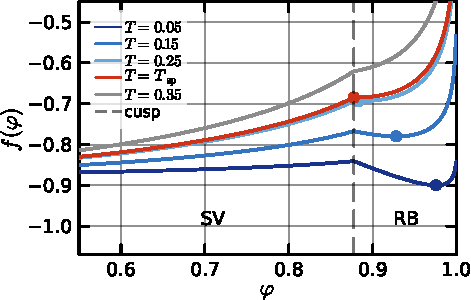
\includegraphics[width=0.82\linewidth]{panels_paper/cusp_illustration.pdf}
\caption{Leading-order free energy per spin $F(\varphi_1)/N$
from~\eqref{eq:F-LO} at $\alpha = 0.50$, $\Bnet = 1$, for several $T$.
The cusp at $\varphi_c = \alpha + \gmax \approx 0.877$ is the boundary
between the retrieval branch (slope $-1$) and the noise-floor branch
(slope $0$).  Dots: basin minima $\phieq(T)$.  At
$T = T_{\mathrm{sp}}(0.50, 1) \approx 0.262$ the minimum reaches the
cusp; above this $T$ the basin no longer exists.}
\label{fig:cusp}
\end{figure}

% =========================================================================
\section{Monte Carlo schemes}
\label{sec:mc}

All chains run on the $\sqrt N$-sphere at $\Bnet = 1$ with Metropolis
updates.  The variants differ in how they handle the $M = \e^{\alpha N}$
patterns.

\paragraph{Direct.}
Store all $M$ patterns explicitly and evaluate~\eqref{eq:lse} over all
of them at every step.  Memory and compute cost $\sim M N$.  Feasible up
to $N \approx 25$ at $\alpha \approx 0.7$ ($M \approx 4 \times 10^7$);
impossible at $N = 100$, $\alpha = 0.6$ ($M \approx 10^{26}$).

\paragraph{Truncated.}
Generate only the patterns with overlap $\varphi_{1\mu} > \varphi_{\mathrm{keep}}$
to the target $\bxi^1$.  The cutoff is chosen so the expected count above
it equals a budget $K \sim 10^4$; the actual count is Poisson with mean
$M \cdot \Pr(\varphi > \varphi_{\mathrm{keep}})$, and the $K$ overlap
values are drawn from the Beta tail.  The patterns below
$\varphi_{\mathrm{keep}}$ are not generated; their contribution enters
the LSE log-sum as the analytic constant
$\ln C_{\mathrm{bulk}} = \alpha N + \ln \int_{-1}^{\varphi_{\mathrm{keep}}}
f(\varphi)\,\e^{N \varphi}\,\dd\varphi$.  The retained set is fixed once
per disorder.  Truncated MC at $N = 25$ matches direct MC on the basin
boundary across the full $\alpha$ range we measure, so the
$\varphi < \varphi_{\mathrm{keep}}$ patterns are genuinely unnecessary
for the basin physics, not silently dropped.  We use truncated for the
wide heatmap.

\paragraph{Hybrid.}
Same kept-tail + analytic-bulk decomposition as truncated, with two
changes: the cutoff is fixed \emph{at the cusp position} $\varphi_c(\alpha,
\Bnet) = [\alpha + \gmax(\Bnet)]/\Bnet$ from~\eqref{eq:F-LO} rather than
chosen by budget, and the bulk integral is evaluated by its
saddle~\eqref{eq:gmax} instead of numerically.  Patterns with
$\varphi_{1\mu} > \varphi_c$ are kept live; the contribution of those
with $\varphi_{1\mu} < \varphi_c$ enters the LSE log-sum as the
$\bx$-independent number $M\,\e^{N \gmax(\Bnet)}$ (state-independent by
rotational symmetry of random patterns, after averaging over their
orthogonal directions to $\bxi^1$).

The live count $K_{\mathrm{cusp}}$ is drawn from a Poisson with mean
$M \cdot \Pr_f(\varphi > \varphi_c)$.  Live overlap values are sampled
from the spherical density~\eqref{eq:exact-density} restricted to
$\varphi > \varphi_c$.  In the rescaled variable $y = (1 + \varphi)/2$
on $[0, 1]$, \eqref{eq:exact-density} becomes
$\mathrm{Beta}((N\!-\!1)/2,\,(N\!-\!1)/2)$ — the change of variable
$(1 - \varphi^2)^{(N-3)/2}\dd\varphi \propto
[y(1-y)]^{(N-3)/2}\dd y$ — so we sample
\begin{equation}
y \sim \mathrm{Beta}\!\Bigl(\tfrac{N\!-\!1}{2},\,\tfrac{N\!-\!1}{2}\Bigr)
   \;\text{truncated to}\; y \in [(1 + \varphi_c)/2,\,1],
\qquad
\varphi_{1\mu} = 2y - 1,
\label{eq:beta-tail}
\end{equation}
which standard libraries provide directly.  Each live pattern is
constructed from $\varphi_{1\mu}$ and a uniform direction $u_\mu$ on the
$(N\!-\!2)$-sphere perpendicular to $\bxi^1$:
$\bxi^\mu = \sqrt N\,\bigl(\varphi_{1\mu},\,\sqrt{1 - \varphi_{1\mu}^2}\,
u_\mu\bigr)$ in the basis where $\bxi^1 = (\sqrt N, 0, \ldots, 0)$.
The live set is fixed once per disorder.

Metropolis runs on the full spin $\bx \in \sqrt N \cdot S^{N-1}$:
Gaussian proposal $\bx' = \bx + \sigma \boldsymbol\eta$ projected back
to $|\bx'| = \sqrt N$; energy
$H(\bx) = -\Bnet^{-1} \ln\!\bigl[\e^{\Bnet\,\bxi^1\!\cdot\!\bx}
+ \sum_{\mu=2}^{K_{\mathrm{cusp}}+1}\!\e^{\Bnet\,\bxi^\mu\!\cdot\!\bx}
+ M\,\e^{N \gmax(\Bnet)}\bigr]$.  Cost per step
$O(K_{\mathrm{cusp}} \cdot N)$.

Crucially the bulk being a constant in $\bx$ does not make the free
energy constant in $\varphi_1$: the chain still feels the sphere
geometry, and below the cusp~\eqref{eq:F-LO} gives
$F(\varphi_1)/N = -\varphi_c - (T/2) \ln(1 - \varphi_1^2)$, which is
minimised at $\varphi_1 = 0$.  Once the chain crosses the cusp it slides
toward $\varphi_1 = 0$ under this entropic attraction; that slide is
what we use to detect basin escape (Sec.~\ref{sec:results}).

At $N = 100$ the spherical density falls fast enough that the expected
$K_{\mathrm{cusp}}$ at the cusp is below $1$ for every $\alpha \in [0.5,
0.62]$ we measure.  The algorithm therefore keeps only $\bxi^1$ explicit
and the bulk constant carries the rest — the chain samples the
leading-order partition function~\eqref{eq:F-LO} directly, with no
$1/N$ subleading corrections.

\paragraph{Why naive ``smart'' fails.}
A faster variant — ``smart'' — refreshes its $K$ kept patterns every
$N_{\mathrm{REFRESH}}$ steps from a cone around the current chain.  This
breaks the quenched-disorder assumption.  As the chain wanders, fresh
patterns are minted at every refresh; the total set of distinct patterns
seen along one trajectory exceeds $M$, and the chain effectively faces a
larger pattern set than the model defines.  Near the retrieval basin the
extra competitors destroy the basin.  Both truncated and hybrid avoid
the problem: the retained set is fixed once per disorder, no refresh.

% =========================================================================
\section{Results}
\label{sec:results}

We measure two observables at $N = 100$:
the mean first-passage escape time $\tau$ from the retrieval basin, and
the steady-state $\avg{\varphi_1} - \phieq(T)$ residual.

\paragraph{Escape time.}
\Cref{fig:tau} reports $\log_{10} \avg{\tau}$ vs $T$ at $N = 100$ for
five $\alpha$ values from the N-dim hybrid MC, averaged over $32$
disorders, with a budget cap at $10^6$ MC steps.  Each curve is a basin
escape profile: at low $T$ the basin is stable for the full budget
(upward triangles at the ceiling); above a critical
$T_{\mathrm{esc}}(\alpha)$ the escape time drops by several orders of
magnitude over a $T$ window of width $\sim 0.01$.  $T_{\mathrm{esc}}$
moves to lower $T$ as $\alpha$ rises; extrapolating to $\tau \to \infty$
at $T = 0$ gives a critical load near $\alpha = 1 - \gmax \approx
0.6226$.

\begin{figure}[t]
\centering
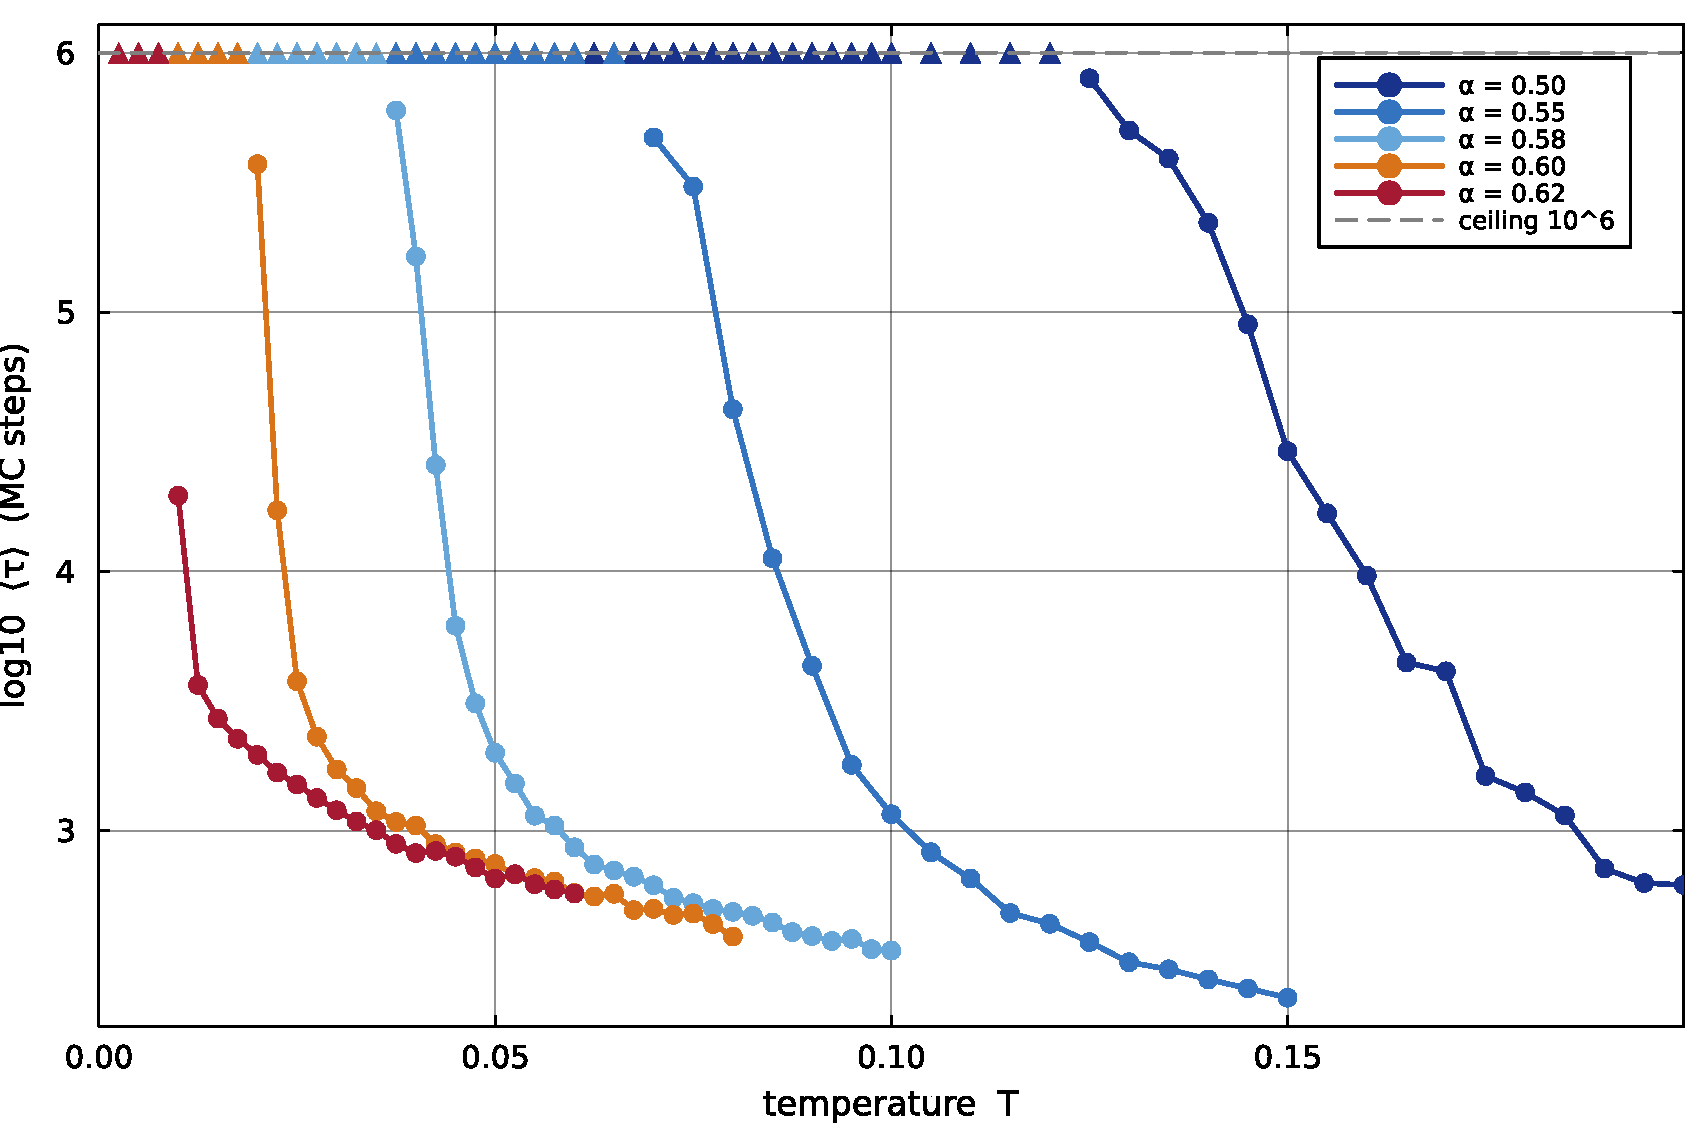
\includegraphics[width=0.82\linewidth]{panels_paper/log_tau_vs_T_N100_Ndim.pdf}
\caption{Mean basin escape time $\avg{\tau}$ vs $T$ at $N = 100$ from
N-dim hybrid MC, $32$ disorders, $\Bnet = 1$.  Five $\alpha$ values:
$0.50, 0.55, 0.58, 0.60, 0.62$.  Filled circles: mean over disorders
that escaped within $10^6$ MC steps.  Upward triangles at
$\log_{10} \tau = 6$: cells where no disorder escaped (lower bound
only).  The escape curve slides toward $T = 0$ as
$\alpha \to 1 - \gmax \approx 0.6226$.}
\label{fig:tau}
\end{figure}

\paragraph{Residual heatmap.}
\Cref{fig:heatmap} shows $\avg{\varphi_1} - \phieq(T)$ over the
$(\alpha, T)$ plane.  Background: truncated MC at varying $N$ over
$\alpha \in [0.20, 0.70]$.  Grey rectangle: N-dim hybrid MC at $N = 100$
on a fine $T$ grid in $\alpha \in [0.50, 0.62]$, $T \in [0, 0.10]$.
The basin (white) is bounded by a sharp transition (dark red) that
follows the saddle line $\acSd(T)$ and pinches at $\alpha \approx
0.6226$, $T = 0$.

\begin{figure}[t]
\centering
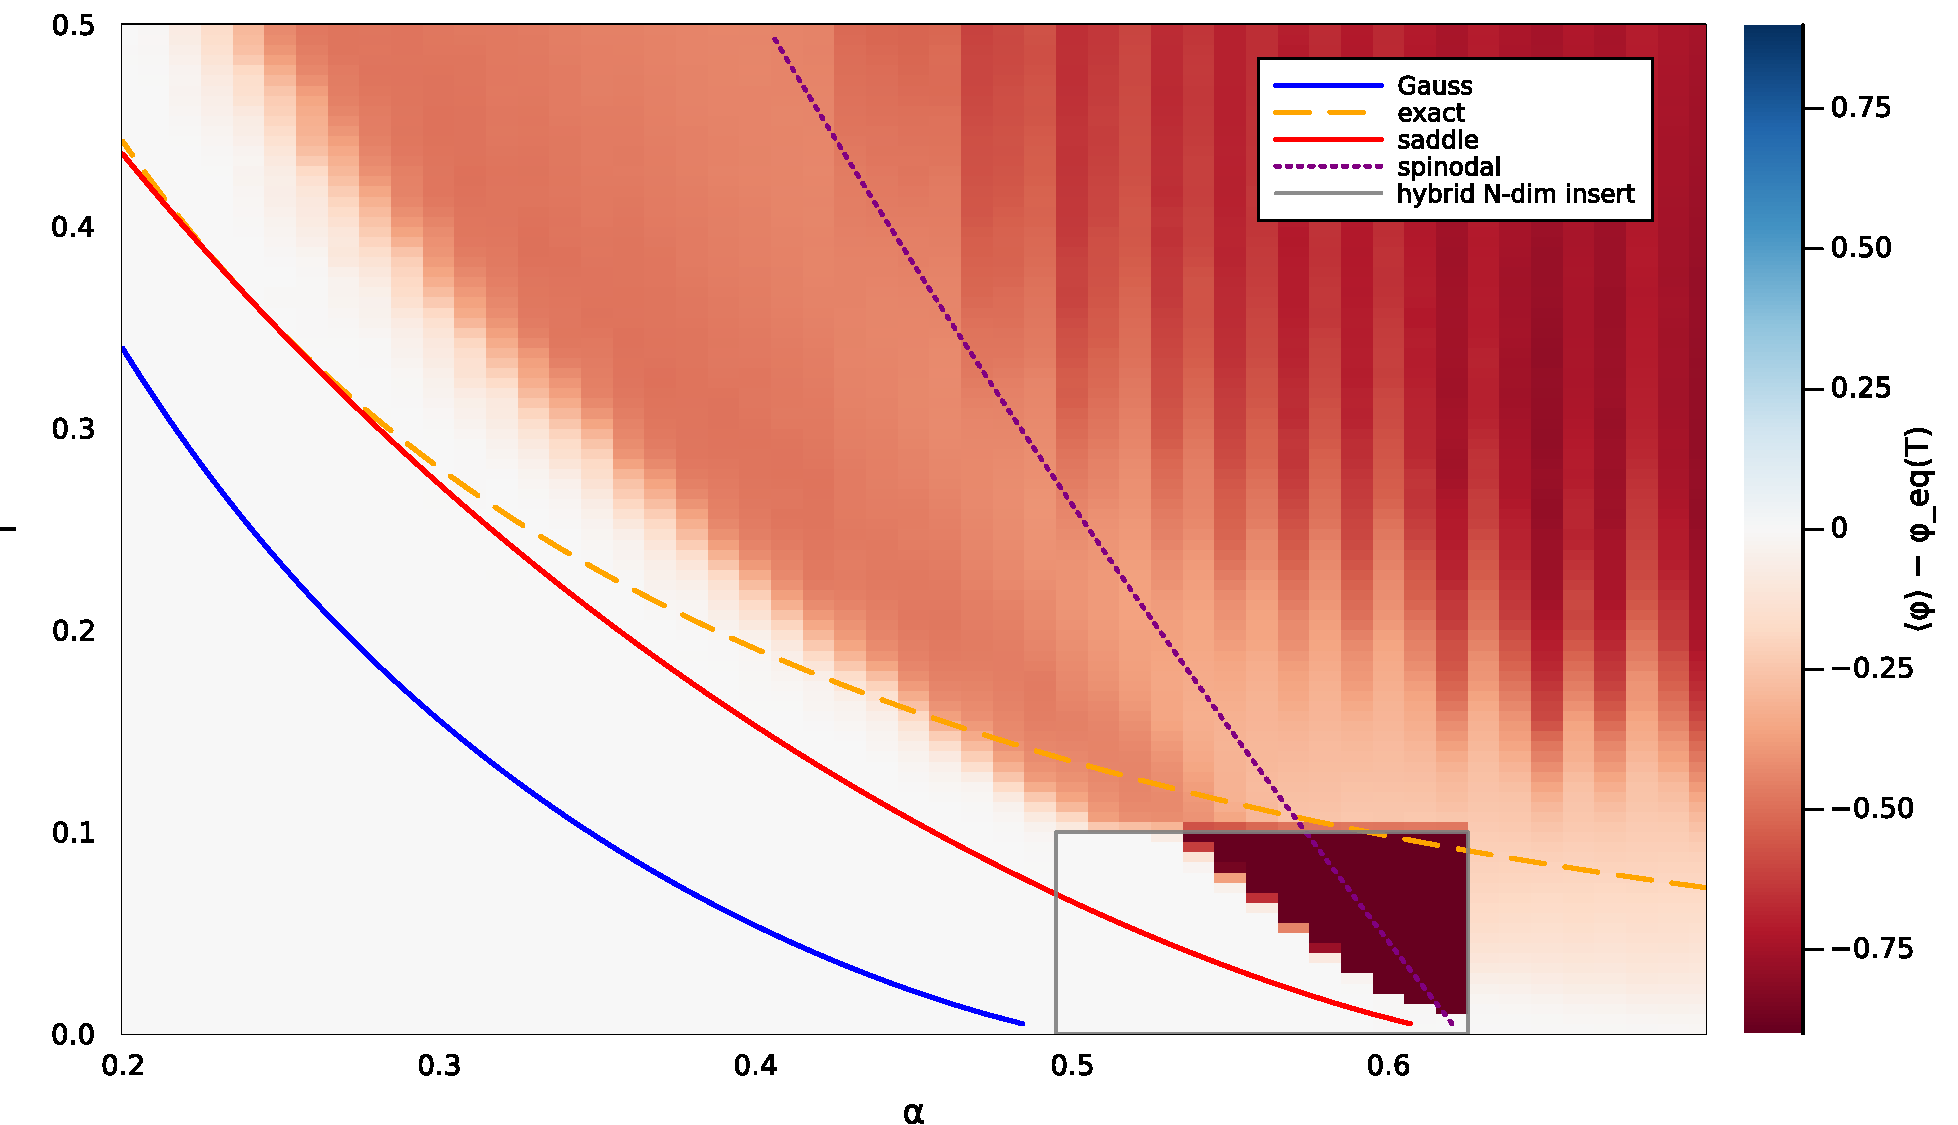
\includegraphics[width=0.98\linewidth]{panels_paper/heatmap_honest_over_Nramp_N100_Ndim.pdf}
\caption{$\avg{\varphi_1} - \phieq(T)$ from Monte Carlo over the
$(\alpha, T)$ plane.  Curves: $\acGauss(T)$ (blue solid,
Eq.~\ref{eq:acgauss}, Gaussian density + support edge); $\acBd(T)$
(orange dashed, Eq.~\ref{eq:acbd}, exact density + support edge);
$\acSd(T)$ (red solid, Eq.~\ref{eq:acsd}, exact density + interior
saddle, this work); $\acSp(T)$ (purple dotted, Eq.~\ref{eq:acsp},
single-pattern spinodal).  Background: truncated MC at varying $N$
over the full $\alpha$ range, linearly interpolated to the fine $T$
grid.  Grey rectangle: N-dim hybrid MC at $N = 100$ on the fine $T$
grid.  The basin pinches at $\alpha \approx 0.6226$ — Ramsauer's
$\acGauss(0) = 1/2$ undershoots by $0.12$ in $\alpha$, a factor $1.25$
in capacity.}
\label{fig:heatmap}
\end{figure}

% =========================================================================
\section{Discussion}
\label{sec:discussion}

The Ramsauer threshold $\alpha_c = 1/2$ is a Gaussian artefact.  The
Gaussian density misses the interior saddle of the partition-sum
integrand~\eqref{eq:Sint} that the exact spherical density places at
$\varphi^{*}(\Bnet)$.  Including it gives
$\alpha_c(\Bnet, 0) = \Bnet - \gmax(\Bnet)$; at the value $\Bnet = 1$
used in our MC, $\alpha_c \approx 0.6226$, a factor $1.25$ larger than
Ramsauer's $1/2$.  The shift is per spin, not asymptotic: it appears at
leading order in $N$ and is visible already at $N = 100$.  A second
signature of the artefact is that Ramsauer's $1/2$ is
$\Bnet$-independent, while the exact-density~\eqref{eq:acsd}
boundary is not.

Open items.
(i) Hot init.  All present runs start the chain at $\bxi^1$ (cold).  The
basin boundary they trace is the spinodal, not the thermodynamic
crossover; hot init at the same grid would delimit the metastability
band.
(ii) Cusp rounding at finite $N$.  The leading-order $\max(\cdot,\cdot)$
in~\eqref{eq:F-LO} is rounded on a scale $1/N$ in $\varphi_1$.  Near the
endpoint $(0.6226, 0)$ the basin offset $\phieq(T) - (\alpha + \gmax)$
falls inside the rounding window, and the leading-order spinodal slope
needs an NLO correction.
(iii) Heatmap consolidation.  \Cref{fig:heatmap} stitches three data
sources.  A clean version would use a single MC variant — truncated with
a hybrid insert near the cusp — across the entire $(\alpha, T)$ plane.

% =========================================================================
\bibliographystyle{plain}
\bibliography{refs}

\end{document}
